% !TEX encoding = UTF-8 Unicode

\documentclass[a4paper]{article}

\usepackage{color}
\usepackage{url}
\usepackage[T2A]{fontenc} % enable Cyrillic fonts
\usepackage[utf8]{inputenc} % make weird characters work
\usepackage{graphicx}

\usepackage[english,serbian]{babel}
%\usepackage[english,serbianc]{babel} %ukljuciti babel sa ovim opcijama, umesto gornjim, ukoliko se koristi cirilica

\usepackage[unicode]{hyperref}
\hypersetup{colorlinks,citecolor=green,filecolor=green,linkcolor=blue,urlcolor=blue}

%\newtheorem{primer}{Пример}[section] %ćirilični primer
\newtheorem{primer}{Primer}[section]

\begin{document}

\title{Should knoweledge be free\\ \small{Seminarski rad u okviru kursa\\Računarstvo i društvo\\ Matematički fakultet}}

\author{Luka Bura 218/2019\\ lukabura89@gmail.com}
\date{3.~april 2023.}
\maketitle

\abstract{

Diskusija ovog seminara se fokusira na prednosti slobodnog i besplatnog znanja i njegove osnovne osobine. Ostale teme uključuju istoriju i razvoj slobodnog znanja, demokratizaciju znanja, etiku, ljudska prava i privatnost na internetu. Takođe, bavićemo se i sajtom Sci-Hub, autora Aleksandre Elbakjan. Besplatno znanje ima mnogo prednosti, ali ne promoviše aktivno alternativne finansijske i distributivne modele, koji bi bili neophodni za postizanje jedinstvenog standarda izvrsnosti za akademsko istraživanje i nastavu.



\tableofcontents



\newpage

\setlength{\parskip}{2em}


\section{Uvod}
\label{sec:uvod}


Pitanje ,,Da li znanje treba da bude besplatno?" je  veoma aktuelno u današnjem svetu. Sa razvojem veštačke inteligencije, interneta i novih tehnologije, pristup informacijama postaje veći, odnosno vrlo lako može da se pronađu odgovori na internetu, što otvara brojna pitanja o tome kako znanje treba da se distribuira i finansira. Dotaći ćemo se online platforme po imenu Sci-Hub, osnivačice Aleksandre Elbakjan i videćemo razne prednosti koje nam ova platforma donosi. Ovaj seminarski rad će se fokusirati na argumente za besplatno znanje i njihove prednosti, istražujući istorijat i razvoj ovog koncepta,neka dodatna etnička pitanja, demokratizaciju znanja, inovaciju tehnologija, humanitarne svrhe i bezbednost na internetu. 


\setlength{\parskip}{2em}



\section{Istorijat i razvoj besplatnog znanja}
\label{sec:istorijat i razvoj besplatnog znanja}


Istorijat besplatnog znanja seže unazad do raznih istorijskih perioda i kulturnih pokreta. U antičkoj Grčkoj, na primer, znanje je često bilo široko dostupno kroz javne debate, dijaloge i biblioteke, kao što je čuvena Biblioteka u Aleksandriji. Tokom renesanse i prosvetiteljstva, znanje je postalo sve dostupnije široj javnosti, delimično zahvaljujući razvoju štampe i popularizaciji naučnih i filozofskih ideja.

U novijoj istoriji, razvoj besplatnog znanja je bio usko povezan sa tehnološkim inovacijama, kao što su kompjuteri, internet i digitalni mediji. Tim ljudi koji je osmislio "World Wide Web", imao je viziju otvorenog, globalnog sistema informacija koji bi omogućio slobodan pristup znanju za sve. Ovaj ideal je doveo do stvaranja mnogih projekata i inicijativa koje se zalažu za besplatno znanje, kao što su Wikipedija, otvoreni pristup, otvoreno obrazovanje i otvoreni podaci.

U poslednjih nekoliko decenija, besplatno znanje je doživelo značajan rast i širenje, zahvaljujući digitalizaciji, veštačkoj inteligenciji, globalizaciji i razvoju informacionih i komunikacionih tehnologija. Ove promene su omogućile širok spektar korisnika da pristupe informacijama i resursima koji su ranije bili dostupni samo uskom krugu akademika, istraživača i stručnjaka.
Međutim, razvoj besplatnog znanja takođe nosi sa sobom brojne izazove i dileme, kao što su pitanja autorskih prava, finansiranja, kvaliteta informacija i digitalne pismenosti. Kako besplatno znanje nastavlja da se širi i razvija, važno je razmotriti ove izazove i raditi na pronalaženju održivih i pravednih rešenja za budućnost globalne razmene znanja.

\setlength{\parskip}{1em}


\begin{verbatim}

\end{verbatim}

\begin{center}
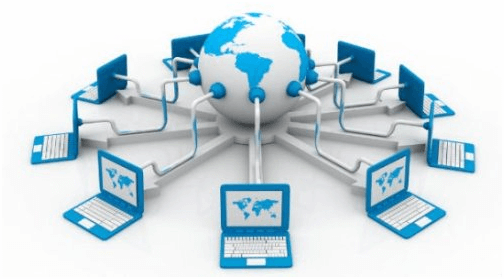
\includegraphics[scale=0.4]{world-wide-web.png}
\end{center}
\caption{Slika 1: World Wide Web}
\label{world wide web}

\setlength{\parskip}{1em}


\section{Sci-Hub}	
\label{sec:sci-hub}

Sci-Hub, osnovan 2011. godine od strane kazahstanske programerke i istraživačice Aleksandre Elbakjan, predstavlja važan primer besplatnog znanja u praksi. Ova platforma omogućava korisnicima besplatan pristup milionima naučnih članaka i knjiga, zaobilazeći tradicionalne pretplate na časopise i autorska prava. Sci-Hub je postao izuzetno popularan među istraživačima širom sveta, naročito u zemljama u razvoju, koje često nemaju sredstava da finansiraju pristup skupim naučnim časopisima.

Sci-Hub je pokrenuo brojne diskusije o pravu na pristup znanju i etičkim pitanjima koja proizilaze iz masovne distribucije zaštićenih radova. Neki smatraju da Sci-Hub doprinosi demokratizaciji znanja, jer omogućava širok spektar korisnika da pristupe najnovijim naučnim otkrićima, bez obzira na njihovu pozadinu ili ekonomske mogućnosti.

Međutim, Sci-Hub takođe suočava se sa kritikama koje se tiču kršenja autorskih prava i potencijalnog negativnog uticaja na naučne izdavače i autore. Neki naučnici i izdavači smatraju da neovlašćeni pristup i distribucija radova podriva ekonomski model naučnog izdavaštva i može dovesti do smanjenja ulaganja u istraživanje i razvoj.

Uprkos ovim izazovima, slučaj Sci-Hub-a ukazuje na rastuću potrebu za promišljanjem o modelima distribucije znanja koji su pravedniji i dostupniji široj javnosti. Ovaj slučaj može poslužiti kao polazište za razmatranje alternativnih modela finansiranja naučnih radova, kao što su otvoreni pristup, hibridni modeli izdavaštva ili državno finansiranje istraživanja, koji mogu osigurati slobodan pristup znanju, dok istovremeno štite interese autora i izdavača. Trenutno se vodi globalna debata oko Sci-Hub-a i ljudi se dele na one koji su za i protiv, malo ima uzdržanih.

\setlength{\parskip}{2em}


\begin{verbatim}

\end{verbatim}

\begin{center}
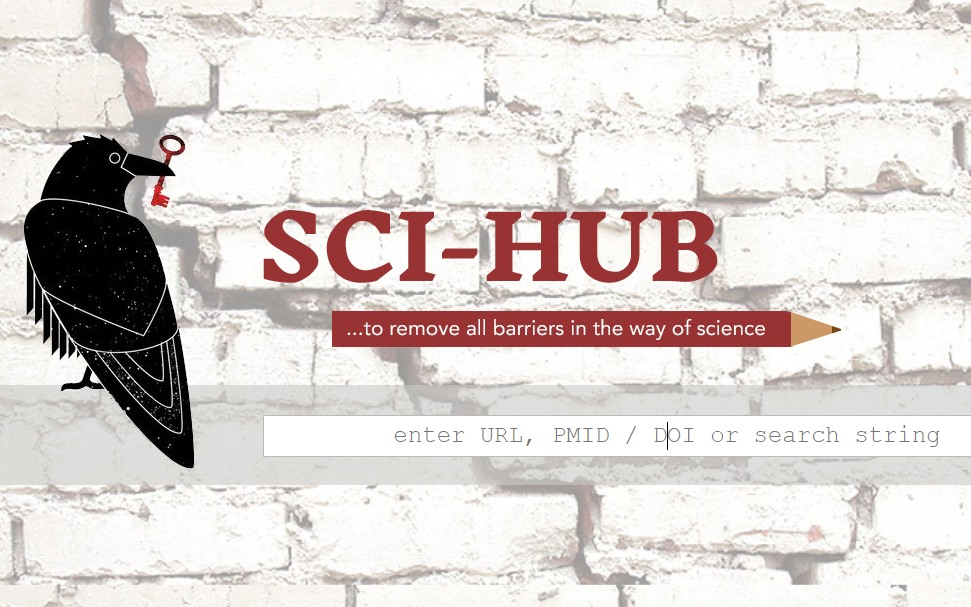
\includegraphics[scale=0.3]{scihub.jpg}
\end{center}
\caption{Slika 2: Sci-Hub}
\label{sci-hub}


\setlength{\parskip}{1em}


\section{Etnička pitanja i jednakost pristupa}
\label{Etnička pitanja i jednakost pristupa}


Besplatno znanje ima značajan uticaj na etnička pitanja i jednakost pristupa informacijama. Kroz pružanje jednakih mogućnosti za pristup znanju, besplatni resursi mogu pomoći u smanjenju nejednakosti među različitim etničkim i socijalnim grupama. Ovo je posebno važno u multikulturalnim društvima i zemljama u razvoju, gde postoje značajne razlike u obrazovanju, ekonomskim mogućnostima i pristupu informacijama.

Besplatni resursi i otvoreni pristup omogućavaju manjinskim grupama i pojedincima iz različitih etničkih sredina da pristupe visokokvalitetnim obrazovnim materijalima, istraživanjima i informacijama koje su im neophodne za obrazovanje i napredovanje u karijeri. To može doprineti smanjenju obrazovnih i ekonomskih jaza među različitim etničkim grupama, kao i stvaranju inkluzivnijeg i pravednijeg društva.

Jednakost pristupa znanju takođe može podstaći raznolikost u naučnim istraživanjima i inovacijama. Kada istraživači iz različitih etničkih i kulturnih pozadina imaju pristup istim informacijama, oni mogu doneti nove perspektive i ideje koje mogu doprineti unapređenju nauke i tehnologije. To može dovesti do stvaranja boljih rešenja za globalne probleme i izazove, kao što su klimatske promene, siromaštvo ili zdravstvena pitanja.
Međutim, važno je razmotriti i izazove koji se tiču jednakosti pristupa znanju i etničkih pitanja. Na primer, potrebno je osigurati da besplatni resursi budu dostupni na različitim jezicima, kako bi se omogućilo što širem spektru korisnika da pristupe informacijama. Takođe, važno je unaprediti digitalnu pismenost među različitim etničkim grupama, kako bi se osiguralo da svi korisnici mogu efikasno koristiti dostupne resurse i informacije.



\setlength{\parskip}{1em}

\section{Inovacija i napredak nauke}
\label{sec:Inovacija i napredak nauke}


Besplatno znanje ima ključnu ulogu u podsticanju inovacija i napretka nauke. Pristup otvorenim izvorima informacija omogućava naučnicima, istraživačima i studentima širom sveta da sarađuju, razmenjuju ideje, unapređuju svoje veštine i stvaraju nova znanja. Osim toga, kroz ovakav pristup, smanjuje se vreme potrebno za pronalaženje relevantnih informacija, što ubrzava naučni razvoj.

Slobodan pristup naučnim radovima i istraživanjima često vodi do interdisciplinarnih otkrića i inovacija, jer omogućava stručnjacima iz različitih oblasti da sarađuju i kombinuju svoje ekspertize. Na primer, istraživači iz oblasti biologije mogu se povezati sa stručnjacima iz računarskih nauka kako bi zajedno razvili nove metode analize genetskih podataka.

Jedan od najpoznatijih primera uspeha besplatnog znanja je projekat Human Genome Project (HGP), međunarodni naučni poduhvat koji je imao za cilj da sektvenira ljudski genom. Rezultati ovog projekta su besplatno dostupni naučnicima širom sveta, što je dovelo do značajnih medicinskih otkrića, razvoja novih terapija i boljeg razumevanja ljudske genetike.

Takođe, besplatno znanje može unaprediti obrazovanje i naučni rad u zemljama u razvoju, koje često nemaju resurse za finansiranje pretplata na naučne časopise i pristup plaćenim izvorima informacija. Ovakav pristup omogućava istraživačima iz ovih zemalja da učestvuju u globalnoj razmeni znanja, čime se podstiče napredak nauke na globalnom nivou.

Uprkos mnogim prednostima, besplatno znanje takođe donosi i izazove, kao što su očuvanje kvaliteta naučnih radova i zaštita intelektualne svojine. Budući da je inovacija i napredak nauke od suštinskog značaja za društvo, neophodno je razmotriti različite modele finansiranja i distribucije znanja kako bi se postigla veća dostupnost i jednakost pristupa, dok se istovremeno osigurava održivost i kvalitet naučnih radova i istraživanja.


\setlength{\parskip}{2em}

\section{Humanitarne svrhe}
\label{Humanitarne svrhe}


Besplatno znanje takođe ima važnu ulogu u rešavanju globalnih problema i humanitarnih kriza. Pristup besplatnim informacijama i istraživanjima može pomoći u pronalaženju rešenja za probleme poput siromaštva, bolesti i klimatskih promena. Takođe, besplatno znanje može doprineti razvoju zdravstvenih usluga i obrazovanja u nerazvijenim i siromašnim zemljama.


\setlength{\parskip}{1em}

\section{Demokratizacija znanja}
\label{Demokratizacija znanja}

Demokratizacija znanja odnosi se na proces širenja znanja i informacija među širokim spektrom ljudi, bez obzira na njihovu pozadinu, obrazovanje ili ekonomski status. Besplatno znanje igra ključnu ulogu u ovom procesu, jer omogućava jednak pristup informacijama koje su ranije bile rezervisane samo za privilegovane pojedince ili institucije.

Jedan od glavnih aspekata demokratizacije znanja je smanjenje socijalnih, ekonomskih i geografskih barijera koje sprečavaju pristup informacijama. Kroz besplatno znanje, ljudi iz siromašnih ili udaljenih područja mogu imati pristup najnovijim naučnim istraživanjima i obrazovnim materijalima, što im omogućava da unaprede svoje veštine i znanje.

Takođe, demokratizacija znanja podstiče uključivanje građana u proces donošenja odluka. Kroz slobodan pristup informacijama, građani mogu bolje razumeti naučne teme, društvena pitanja i političke procese, čime se poboljšava transparentnost i odgovornost vlasti. Ovaj aspekt demokratizacije znanja posebno je važan u zemljama u razvoju, gde pristup informacijama može pomoći u borbi protiv korupcije i unapređenju demokratskih institucija.

Demokratizacija znanja takođe može doprineti većoj raznolikosti u naučnim istraživanjima, jer omogućava istraživačima iz različitih kultura, etničkih grupa i društvenih sredina da sarađuju i razmenjuju ideje. Ovo može dovesti do novih perspektiva, pristupa i rešenja koja možda ne bi bila moguća bez širokog pristupa znanju.

Iako demokratizacija znanja ima mnoge prednosti, postoje i izazovi koji se moraju razmotriti. Na primer, potrebno je razvijati mehanizme za zaštitu autorskih prava i intelektualne svojine, kako bi se očuvala kvaliteta naučnih radova i istraživanja. Takođe, važno je pronaći održive modele finansiranja i distribucije znanja kako bi se osigurala dostupnost i jednakost pristupa informacijama.


\begin{verbatim}

\end{verbatim}

\begin{center}
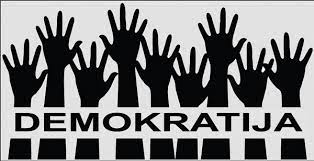
\includegraphics[scale=0.85]{demokratija.jpeg}
\end{center}
\caption{Slika 3: Demokratija}
\label{demokratija}


\setlength{\parskip}{1em}

\section{Bezbednost na internetu}
\label{Bezbednost na internetu}


Pitanje bezbednosti na internetu je važno u kontekstu besplatnog znanja, jer se često koriste digitalni resursi za deljenje informacija i istraživanja. Besplatno znanje zahteva razvijanje mehanizama za zaštitu intelektualne svojine, autorskih prava i privatnosti korisnika, dok istovremeno omogućava širok pristup informacijama. Jedan od primera nebezbednih sajtova sa vrlo širokim opusom informacija je Wikipedija. Većina ljudi odmah potraži informacije na Wikipediji, ali treba naglasiti da Wikipediju može da uređuje gotovo ko želi, tako da tačnost tih informacija nije zasigurno proverena. Osim Wikipedije, razni medijski članci nisu skroz pouzdani, pa ne treba ni njima zasigurno verovati. Najbolje je pronaći neki rad, koji ima puno recenzenata, puno dobrih ocena, lepih komentara, koji nam ukazuju na validnost tog sajta, odnosno naučnog rada. 


\setlength{\parskip}{1em}

\section{Sloboda govora}
\label{Sloboda govora}

Tema "Da li znanje treba da bude besplatno?" u kontekstu slobode govora postavlja brojna važna pitanja o pravima i obavezama pojedinaca i društva. Sloboda govora je fundamentalno pravo koje omogućava razvoj i napredak, ali i nosi izazove u pogledu etike, privatnosti i sigurnosti.

Kada govorimo o besplatnom znanju i slobodi govora, moramo uzeti u obzir potrebu za transparentnošću i otvorenošću u razmeni informacija. U savremenom društvu, gde se tehnologija razvija brzo, pristup informacijama i znanju može biti ključan za rešavanje globalnih izazova, kao što su klimatske promene, socijalna nejednakost i zdravstvene krize.

Međutim, sloboda govora i besplatno znanje takođe mogu dovesti do problema, kao što su širenje lažnih informacija, kršenje autorskih prava i kompromitovanje privatnosti pojedinaca. Kako bi se pronašla ravnoteža između ovih elemenata, društvo mora razmotriti etičke i pravne aspekte kako bi se obezbedila zaštita prava i interesa svih uključenih strana.

Jedno od mogućih rešenja je razvijanje i implementacija jasnih smernica i politika koje će omogućiti pristup znanju i informacijama, dok će istovremeno štititi privatnost i intelektualnu svojinu. Ovo uključuje i unapređenje sistema obrazovanja koji podstiču slobodnu razmenu ideja i kritičko razmišljanje, kao i razvijanje tehnoloških alata koji će osigurati autentičnost i verodostojnost informacija koje se dele.

U suštini, promovisanje slobode govora i besplatnog znanja može dovesti do boljeg razumevanja sveta u kojem živimo i omogućiti rešavanje izazova sa kojima se suočavamo. Međutim, to zahteva odgovoran pristup i neprekidnu pažnju na etičke, pravne i bezbednosne aspekte koji prate ovu slobodu.


\begin{verbatim}

\end{verbatim}

\begin{center}
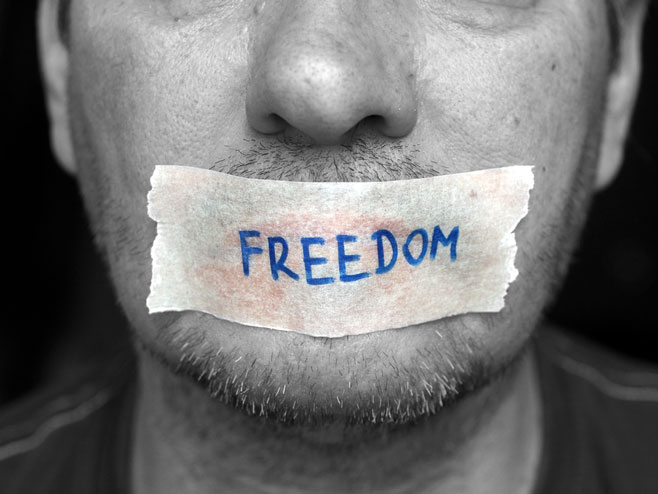
\includegraphics[scale=0.35]{sloboda_govora.jpg}
\end{center}
\caption{Slika 4: Sloboda govora}
\label{Sloboda govora}


\setlength{\parskip}{2em}


\setlength{\parskip}{1em}

\section{Zaključak}
\label{Zaključak}

Besplatno znanje ima mnoge prednosti, uključujući smanjenje socijalnih i etničkih barijera, podsticanje inovacija i napretka nauke, demokratizaciju znanja i doprinos humanitarnim ciljevima. Međutim, važno je razvijati mehanizme koji će osigurati bezbednost na internetu i zaštitu intelektualne svojine. Slučaj Sci-Hub-a pokazuje kako besplatno znanje može imati pozitivan uticaj na naučnu zajednicu, ali i ukazuje na potrebu za balansom između besplatnog pristupa informacijama i zaštite autorskih prava. U budućnosti, neophodno je razmotriti različite modele finansiranja i distribucije znanja kako bi se postigla veća dostupnost i jednakost pristupa, dok se istovremeno osigurava održivost i kvalitet naučnih radova i istraživanja.

\setlength{\parskip}{11em}




\addcontentsline{toc}{section}{Reference}
\appendix

\iffalse
\bibliography{seminarski} 
\bibliographystyle{plain}
\fi

\begin{thebibliography}{9}

\setlength{\parskip}{1em}

\bibitem   a Martin, Mackenzie A. (2016). The sharing economy, the English language and transnational governance.

\bibitem{gcc} Nielsen, M. (2012). Reinventing discovery: The new era of networked science. Princeton University Press.

\bibitem{haltingproblem} Pisani, E., & AbouZahr, C. (2010). Sharing health data: Good intentions are not enough.

\bibitem{haltingproblem} Bohannon, J. (2016). Who's downloading pirated papers? Everyone. Science

\bibitem{haltingproblem} Pisani, E., & AbouZahr, C. (2010). Sharing health data: Good intentions are not enough.

\bibitem{haltingproblem} Greshake, B. (2017). Looking into Pandora's Box: The Content of Sci-Hub and its Usage

\bibitem{haltingproblem} Himmelstein, D. S., Romero, A. R., Levernier, J. G., Munro,T. A., McLaughlin, S. R., Greshake Tzovaras, B., & Greene, C. S. (2018). Sci-Hub provides access to nearly all scholarly literature

\bibitem{haltingproblem} Bauwens, M., & Kostakis, V. (2014). Network society and future scenarios for a collaborative economy 

\bibitem{haltingproblem} Benkler, Y. (2006). The wealth of networks: How social production transforms markets and freedom. Yale University Press.

\bibitem{haltingproblem} Suber, P. (2012). Open access. MIT Press

\bibitem{haltingproblem} 
Chan, L., & Costa, S. (2005). Participation in the global knowledge commons: Challenges and opportunities for research dissemination in developing countries

\bibitem{haltingproblem} Willinsky, J. (2006). The access principle: The case for open access to research and scholarship. MIT Press.

\bibitem{haltingproblem} Casson, L. (2002). Libraries in the ancient world


\end{thebibliography}


\end{document}
